
\chapter{Common logarithm function}
\competences{converting between exponential and logarithmic form, solving, modelling}
\section{Reference notes}
\begin{retenir}
For every $b>0$, $\log(b)$ is the unique real number $x$ such that $10^x=b$. Hence $\log(10^x)=x$ and, for $b>0$, $10^{\log(b)}=b$. The function $\log$ is defined on $]0,+\infty[$ and it is strictly increasing.
\end{retenir}

\begin{center}
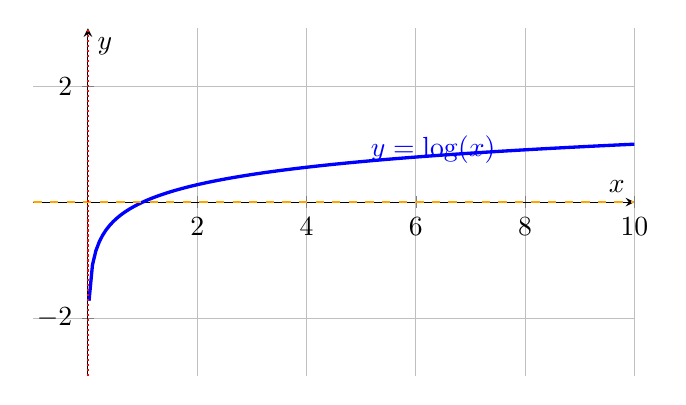
\begin{tikzpicture}
\begin{axis}[width=.76\textwidth,height=6cm,axis lines=middle,xmin=-1,xmax=10,ymin=-3,ymax=3,grid=major,xlabel={$x$},ylabel={$y$}]
\addplot[Blue,very thick,samples=160,domain=.02:10]{ln(x)/ln(10)};
\addplot[Orange,dashed,thick,domain=-1:10]{0};
\addplot[Red,densely dotted,thick] coordinates {(0,-3)(0,3)};
\node[anchor=west,Blue] at (axis cs:5,.9) {$y=\log(x)$};
\end{axis}
\end{tikzpicture}
\end{center}

For $a>0$, $b>0$ and every natural number $n$:
\[
\log(ab)=\log(a)+\log(b),\qquad
\log\!\left(\frac{a}{b}\right)=\log(a)-\log(b),\qquad
\log(a^n)=n\log(a).
\]

\begin{erreur}
$\log(a+b)$ does not simplify. Before any logarithmic calculation, check that each argument is strictly positive.
\end{erreur}

\begin{methode}
To solve $a^x=b$, with $a>0$, $a\neq1$ and $b>0$, take the logarithm: $x\log(a)=\log(b)$, so $x=\dfrac{\log(b)}{\log(a)}$.
\end{methode}

\begin{exemple}
Solving $1.08^x=2$ amounts to writing $x=\dfrac{\log(2)}{\log(1.08)}\approx9.01$. A value multiplied by $1.08$ each year therefore doubles after a little more than nine years.
\end{exemple}

Since $\log$ is increasing, for $a,b>0$, $a<b$ is equivalent to $\log(a)<\log(b)$. For $a>1$, $a^x<b$ is equivalent to $x<\dfrac{\log b}{\log a}$; when $0<a<1$, the inequality sign reverses.

\sessionheader{15}{17 Nov 2026}{B: 2 h -- C: 1 h}{Definition of the common logarithm}{Common logarithm function}
\begin{objectifs}\begin{itemize}\item Link powers of 10 and logarithms.\item Calculate common values.\item Use the calculator.\end{itemize}\end{objectifs}
\begin{automatismes}\begin{enumerate}\item Calculate $20\,\%$ of $80$. \rep{$16$}\item Give the domain of $\log$. \rep{$]0,+\infty[$}\item Calculate $\log(10^4)$. \rep{$4$}\item Solve $10^x=0.01$. \rep{$x=-2$}\item Expand $\log(3b)$, $b>0$. \rep{$\log3+\log b$}\end{enumerate}\end{automatismes}
\begin{prerequis}Reread the last written record and be able to carry out the basic calculations needed today. Before the investigation, have students rephrase the key words: link powers of 10 and logarithms and calculate common values.\end{prerequis}

\begin{activite}
Complete the pairs $10^x=b$ and $x=\log(b)$ for $b=0.001;0.1;1;10;1\,000$. Then use the calculator for $b=7$.

\end{activite}
\enseignant{The logarithms are $-3,-1,0,1,3$; $\log(7)\approx0.8451$. Have students say aloud which piece of data triggers the choice of method.}

\begin{traceecrite}For $b>0$, $\log(b)$ is the unique solution of $10^x=b$. In particular $\log(1)=0$, $\log(10)=1$ and $\log(100)=2$.\end{traceecrite}

\begin{exemple}
Revisit the data from the investigation and write up the solution in order: definition of the objects, property used, exact or approximate calculation, then a concluding sentence. The model answer appears in the teacher edition.
\end{exemple}
\enseignant{The logarithms are $-3,-1,0,1,3$; $\log(7)\approx0.8451$.}

\begin{exercice}[-- essential]
\begin{enumerate}\item Calculate $\log(10^2)$ and $\log(10^{-2})$.\item Expand $\log\!\left(\dfrac{100a^2}{b}\right)$ for $a,b>0$.\item Solve $2^x=22$ and give an approximate value to the nearest hundredth.\end{enumerate}
\end{exercice}
\enseignant{$2$ and $-2$. The expression equals $2+2\log(a)-\log(b)$. Finally $x=\dfrac{\log(22)}{\log(2)}$.}

\manuelref{Calao, course pp. 64--69; exercises p. 70, no.~1--5}
\CalaoSession{15}

\begin{dm}Redo practice exercise 2 with the following data: replace the initial value by $195$ and the rate or common ratio by $5$. Write it up in four lines: data, formula, calculation, conclusion.\end{dm}
\enseignant{The answer depends on the exercise revisited. Check above all the consistency of the model, the number of iterations, the rounding and the concluding sentence.}

\begin{sortie}On a half-sheet: write the main rule of the session, work through a very short example and state your confidence level from 1 to 4. Key question(s) of the day: 1, 2 and 3.\end{sortie}

\ifprof
\begin{methode}
\textbf{1 h session:} 7 min of fluency; 10 min of pooling and written record; 28 min of essential exercises; 5 min of correction; 3 min of exit ticket.\\
\textbf{2 h session:} add 20 min of investigation, 20 min of formalisation, a second independent exercise and 10 min of comparative correction.\\
\textbf{Differentiation:} give struggling students a four-box sheet (data, model, calculation, conclusion). Ask quick students to produce a counterexample, a justification or a second method.
\end{methode}
\fi
\sessionheader{16}{19 Nov 2026}{B: 1 h -- C: 2 h}{Variations and graph}{Common logarithm function}
\begin{objectifs}\begin{itemize}\item Know the domain.\item Use the fact that the function is increasing.\item Read the curve.\end{itemize}\end{objectifs}
\begin{automatismes}\begin{enumerate}\item Write the multiplier for an increase of $25\,\%$. \rep{$1+\dfrac{25}{100}=1.25$}\item Calculate $\log(10^0)$. \rep{$0$}\item Solve $10^x=0.01$. \rep{$x=-2$}\item Expand $\log(3b)$, $b>0$. \rep{$\log3+\log b$}\item Give the domain of $\log$. \rep{$]0,+\infty[$}\end{enumerate}\end{automatismes}
\begin{prerequis}Reread the last written record and be able to carry out the basic calculations needed today. Before the investigation, have students rephrase the key words: know the domain and use the fact that the function is increasing.\end{prerequis}

\begin{activite}
Plot $y=10^x$ and the line $y=x$, then obtain the curve of the logarithm by symmetry. Deduce its domain, its direction of variation and its asymptote.
\begin{center}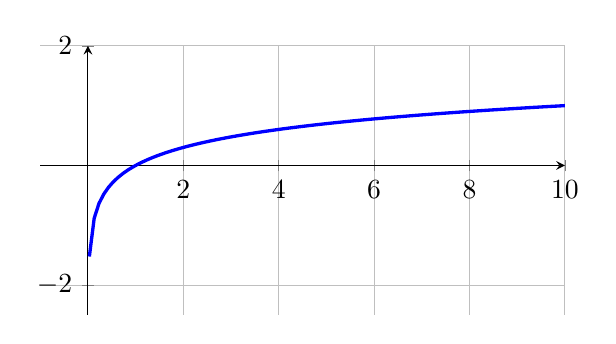
\begin{tikzpicture}\begin{axis}[width=.68\textwidth,height=5cm,axis lines=middle,xmin=-1,xmax=10,ymin=-2.5,ymax=2,grid=major]\addplot[Blue,very thick,samples=100,domain=.03:10]{ln(x)/ln(10)};\end{axis}\end{tikzpicture}\end{center}
\end{activite}
\enseignant{The logarithm is the inverse function of $10^x$: domain $]0,+\infty[$, strictly increasing, asymptote $x=0$. Have students say aloud which piece of data triggers the choice of method.}

\begin{traceecrite}The function $\log$ is defined on $]0,+\infty[$, is strictly increasing, and its curve has $x=0$ as a vertical asymptote.\end{traceecrite}

\begin{exemple}
Revisit the data from the investigation and write up the solution in order: definition of the objects, property used, exact or approximate calculation, then a concluding sentence. The model answer appears in the teacher edition.
\end{exemple}
\enseignant{The logarithm is the inverse function of $10^x$: domain $]0,+\infty[$, strictly increasing, asymptote $x=0$.}

\begin{exercice}[-- essential]
\begin{enumerate}\item Calculate $\log(10^3)$ and $\log(10^{-3})$.\item Expand $\log\!\left(\dfrac{100a^2}{b}\right)$ for $a,b>0$.\item Solve $3^x=23$ and give an approximate value to the nearest hundredth.\end{enumerate}
\end{exercice}
\enseignant{$3$ and $-3$. The expression equals $2+2\log(a)-\log(b)$. Finally $x=\dfrac{\log(23)}{\log(3)}$.}

\manuelref{Calao, course pp. 64--69; exercises p. 70, no.~6--10}
\CalaoSession{16}

\begin{dm}Redo practice exercise 3 with the following data: replace the initial value by $200$ and the rate or common ratio by $6$. Write it up in four lines: data, formula, calculation, conclusion.\end{dm}
\enseignant{The answer depends on the exercise revisited. Check above all the consistency of the model, the number of iterations, the rounding and the concluding sentence.}

\begin{sortie}On a half-sheet: write the main rule of the session, work through a very short example and state your confidence level from 1 to 4. Key question(s) of the day: 1 and 2.\end{sortie}

\ifprof
\begin{methode}
\textbf{1 h session:} 7 min of fluency; 10 min of pooling and written record; 28 min of essential exercises; 5 min of correction; 3 min of exit ticket.\\
\textbf{2 h session:} add 20 min of investigation, 20 min of formalisation, a second independent exercise and 10 min of comparative correction.\\
\textbf{Differentiation:} give struggling students a four-box sheet (data, model, calculation, conclusion). Ask quick students to produce a counterexample, a justification or a second method.
\end{methode}
\fi
\sessionheader{17}{24 Nov 2026}{B: 2 h -- C: 1 h}{Algebraic properties}{Common logarithm function}
\begin{objectifs}\begin{itemize}\item Expand or condense logarithms.\item Check the conditions.\item Avoid false properties.\end{itemize}\end{objectifs}
\begin{automatismes}\begin{enumerate}\item Simplify $3x+6-x+2$. \rep{$2x+8$}\item Solve $10^x=0.01$. \rep{$x=-2$}\item Expand $\log(3b)$, $b>0$. \rep{$\log3+\log b$}\item Give the domain of $\log$. \rep{$]0,+\infty[$}\item Calculate $\log(10^1)$. \rep{$1$}\end{enumerate}\end{automatismes}
\begin{prerequis}Reread the last written record and be able to carry out the basic calculations needed today. Before the investigation, have students rephrase the key words: expand or condense logarithms and check the conditions.\end{prerequis}

\begin{activite}
Starting from $10^2\times10^3=10^5$, conjecture $\log(ab)=\log a+\log b$. Test numerically with $a=2,b=5$, then explain why $a,b$ must be positive.

\end{activite}
\enseignant{$\log(2)+\log(5)=\log(10)=1$. The logarithm is only defined for a strictly positive argument. Have students say aloud which piece of data triggers the choice of method.}

\begin{traceecrite}For $a,b>0$, $\log(ab)=\log a+\log b$ and $\log\!\left(\dfrac ab\right)=\log a-\log b$. Moreover $\log(a^n)=n\log a$.\end{traceecrite}

\begin{exemple}
Revisit the data from the investigation and write up the solution in order: definition of the objects, property used, exact or approximate calculation, then a concluding sentence. The model answer appears in the teacher edition.
\end{exemple}
\enseignant{$\log(2)+\log(5)=\log(10)=1$. The logarithm is only defined for a strictly positive argument.}

\begin{exercice}[-- essential]
\begin{enumerate}\item Calculate $\log(10^4)$ and $\log(10^{-4})$.\item Expand $\log\!\left(\dfrac{100a^2}{b}\right)$ for $a,b>0$.\item Solve $4^x=24$ and give an approximate value to the nearest hundredth.\end{enumerate}
\end{exercice}
\enseignant{$4$ and $-4$. The expression equals $2+2\log(a)-\log(b)$. Finally $x=\dfrac{\log(24)}{\log(4)}$.}

\manuelref{Calao, course pp. 66--69; exercises p. 72, no.~20--23}
\CalaoSession{17}

\begin{dm}Redo practice exercise 2 with the following data: replace the initial value by $205$ and the rate or common ratio by $7$. Write it up in four lines: data, formula, calculation, conclusion.\end{dm}
\enseignant{The answer depends on the exercise revisited. Check above all the consistency of the model, the number of iterations, the rounding and the concluding sentence.}

\begin{sortie}On a half-sheet: write the main rule of the session, work through a very short example and state your confidence level from 1 to 4. Key question(s) of the day: 1, 2 and 3.\end{sortie}

\ifprof
\begin{methode}
\textbf{1 h session:} 7 min of fluency; 10 min of pooling and written record; 28 min of essential exercises; 5 min of correction; 3 min of exit ticket.\\
\textbf{2 h session:} add 20 min of investigation, 20 min of formalisation, a second independent exercise and 10 min of comparative correction.\\
\textbf{Differentiation:} give struggling students a four-box sheet (data, model, calculation, conclusion). Ask quick students to produce a counterexample, a justification or a second method.
\end{methode}
\fi
\sessionheader{18}{26 Nov 2026}{B: 1 h -- C: 2 h}{Solving $10^x=b$}{Common logarithm function}
\begin{objectifs}\begin{itemize}\item Solve $10^x=b$.\item Bracket a solution.\item Interpret an order of magnitude.\end{itemize}\end{objectifs}
\begin{automatismes}\begin{enumerate}\item Calculate $5\,\%$ of $140$. \rep{$7$}\item Expand $\log(3b)$, $b>0$. \rep{$\log3+\log b$}\item Give the domain of $\log$. \rep{$]0,+\infty[$}\item Calculate $\log(10^2)$. \rep{$2$}\item Solve $10^x=0.01$. \rep{$x=-2$}\end{enumerate}\end{automatismes}
\begin{prerequis}Reread the last written record and be able to carry out the basic calculations needed today. Before the investigation, have students rephrase the key words: solve $10^x=b$ and bracket a solution.\end{prerequis}

\begin{activite}
A device measures intensities $b=0.04;3.2;850$. For each value, solve $10^x=b$, give $x$ to the nearest hundredth and check by calculating $10^x$.

\end{activite}
\enseignant{$x=\log(b)$: approximately $-1.40$, $0.51$ and $2.93$. Have students say aloud which piece of data triggers the choice of method.}

\begin{traceecrite}The equation $10^x=b$ has a solution only if $b>0$; this solution is $x=\log(b)$.\end{traceecrite}

\begin{exemple}
Revisit the data from the investigation and write up the solution in order: definition of the objects, property used, exact or approximate calculation, then a concluding sentence. The model answer appears in the teacher edition.
\end{exemple}
\enseignant{$x=\log(b)$: approximately $-1.40$, $0.51$ and $2.93$.}

\begin{exercice}[-- essential]
\begin{enumerate}\item Calculate $\log(10^5)$ and $\log(10^{-5})$.\item Expand $\log\!\left(\dfrac{100a^2}{b}\right)$ for $a,b>0$.\item Solve $5^x=25$ and give an approximate value to the nearest hundredth.\end{enumerate}
\end{exercice}
\enseignant{$5$ and $-5$. The expression equals $2+2\log(a)-\log(b)$. Finally $x=\dfrac{\log(25)}{\log(5)}$.}

\manuelref{Calao, p. 73, no.~30--32}
\CalaoSession{18}

\begin{dm}Redo practice exercise 3 with the following data: replace the initial value by $210$ and the rate or common ratio by $2$. Write it up in four lines: data, formula, calculation, conclusion.\end{dm}
\enseignant{The answer depends on the exercise revisited. Check above all the consistency of the model, the number of iterations, the rounding and the concluding sentence.}

\begin{sortie}On a half-sheet: write the main rule of the session, work through a very short example and state your confidence level from 1 to 4. Key question(s) of the day: 1 and 2.\end{sortie}

\ifprof\clearpage
\begin{methode}
\textbf{1 h session:} 7 min of fluency; 10 min of pooling and written record; 28 min of essential exercises; 5 min of correction; 3 min of exit ticket.\\
\textbf{2 h session:} add 20 min of investigation, 20 min of formalisation, a second independent exercise and 10 min of comparative correction.\\
\textbf{Differentiation:} give struggling students a four-box sheet (data, model, calculation, conclusion). Ask quick students to produce a counterexample, a justification or a second method.
\end{methode}
\fi
\sessionheader{19}{1 Dec 2026}{B: 2 h -- C: 1 h}{Solving $a^x=b$}{Common logarithm function}
\begin{objectifs}\begin{itemize}\item Solve $a^x=b$.\item Use a quotient of logarithms.\item Round sensibly.\end{itemize}\end{objectifs}
\begin{automatismes}\begin{enumerate}\item Write the multiplier for an increase of $10\,\%$. \rep{$1+\dfrac{10}{100}=1.10$}\item Give the domain of $\log$. \rep{$]0,+\infty[$}\item Calculate $\log(10^3)$. \rep{$3$}\item Solve $10^x=0.01$. \rep{$x=-2$}\item Expand $\log(3b)$, $b>0$. \rep{$\log3+\log b$}\end{enumerate}\end{automatismes}
\begin{prerequis}Reread the last written record and be able to carry out the basic calculations needed today. Before the investigation, have students rephrase the key words: solve $a^x=b$ and use a quotient of logarithms.\end{prerequis}

\begin{activite}
The number of subscribers is multiplied by $1.15$ each month. Determine after how many months it will have tripled. Set up the equation, solve it using logarithms and interpret the rounding.

\end{activite}
\enseignant{$1.15^n\geq3$; $\dfrac{\log3}{\log1.15}\approx7.86$. So eight whole months are needed. Have students say aloud which piece of data triggers the choice of method.}

\begin{traceecrite}For $a>0$, $a\neq1$ and $b>0$, $a^x=b$ is equivalent to $x=\dfrac{\log(b)}{\log(a)}$.\end{traceecrite}

\begin{exemple}
Revisit the data from the investigation and write up the solution in order: definition of the objects, property used, exact or approximate calculation, then a concluding sentence. The model answer appears in the teacher edition.
\end{exemple}
\enseignant{$1.15^n\geq3$; $\dfrac{\log3}{\log1.15}\approx7.86$. So eight whole months are needed.}

\begin{exercice}[-- essential]
\begin{enumerate}\item Calculate $\log(10^6)$ and $\log(10^{-6})$.\item Expand $\log\!\left(\dfrac{100a^2}{b}\right)$ for $a,b>0$.\item Solve $6^x=26$ and give an approximate value to the nearest hundredth.\end{enumerate}
\end{exercice}
\enseignant{$6$ and $-6$. The expression equals $2+2\log(a)-\log(b)$. Finally $x=\dfrac{\log(26)}{\log(6)}$.}

\manuelref{Calao, p. 74, no.~33--39}
\CalaoSession{19}

\begin{dm}Redo practice exercise 2 with the following data: replace the initial value by $215$ and the rate or common ratio by $3$. Write it up in four lines: data, formula, calculation, conclusion.\end{dm}
\enseignant{The answer depends on the exercise revisited. Check above all the consistency of the model, the number of iterations, the rounding and the concluding sentence.}

\begin{sortie}On a half-sheet: write the main rule of the session, work through a very short example and state your confidence level from 1 to 4. Key question(s) of the day: 1, 2 and 3.\end{sortie}

\ifprof
\begin{methode}
\textbf{1 h session:} 7 min of fluency; 10 min of pooling and written record; 28 min of essential exercises; 5 min of correction; 3 min of exit ticket.\\
\textbf{2 h session:} add 20 min of investigation, 20 min of formalisation, a second independent exercise and 10 min of comparative correction.\\
\textbf{Differentiation:} give struggling students a four-box sheet (data, model, calculation, conclusion). Ask quick students to produce a counterexample, a justification or a second method.
\end{methode}
\fi
\sessionheader{20}{3 Dec 2026}{B: 1 h -- C: 2 h}{Equations $x^a=b$ and simple inequalities}{Common logarithm function}
\begin{objectifs}\begin{itemize}\item Solve equations where the variable is the base.\item Deal with an inequality.\item Take the domain into account.\end{itemize}\end{objectifs}
\begin{automatismes}\begin{enumerate}\item Simplify $3x+9-x+2$. \rep{$2x+11$}\item Calculate $\log(10^4)$. \rep{$4$}\item Solve $10^x=0.01$. \rep{$x=-2$}\item Expand $\log(3b)$, $b>0$. \rep{$\log3+\log b$}\item Give the domain of $\log$. \rep{$]0,+\infty[$}\end{enumerate}\end{automatismes}
\begin{prerequis}Reread the last written record and be able to carry out the basic calculations needed today. Before the investigation, have students rephrase the key words: solve equations where the variable is the base and deal with an inequality.\end{prerequis}

\begin{activite}
Solve on $[0,+\infty[$: $x^3=40$, then $x^4=16$. Then solve $1.08^x<1.5$ and explain the role of the function being increasing.

\end{activite}
\enseignant{$x=\sqrt[3]{40}\approx3.42$; $x=2$ on the requested interval; $x<\dfrac{\log1.5}{\log1.08}\approx5.27$. Have students say aloud which piece of data triggers the choice of method.}

\begin{traceecrite}To solve $x^n=b$, take the domain and the parity of $n$ into account. For an exponential inequality, the direction depends on whether the function is increasing or decreasing.\end{traceecrite}

\begin{exemple}
Revisit the data from the investigation and write up the solution in order: definition of the objects, property used, exact or approximate calculation, then a concluding sentence. The model answer appears in the teacher edition.
\end{exemple}
\enseignant{$x=\sqrt[3]{40}\approx3.42$; $x=2$ on the requested interval; $x<\dfrac{\log1.5}{\log1.08}\approx5.27$.}

\begin{exercice}[-- essential]
\begin{enumerate}\item Calculate $\log(10^2)$ and $\log(10^{-2})$.\item Expand $\log\!\left(\dfrac{100a^2}{b}\right)$ for $a,b>0$.\item Solve $2^x=22$ and give an approximate value to the nearest hundredth.\end{enumerate}
\end{exercice}
\enseignant{$2$ and $-2$. The expression equals $2+2\log(a)-\log(b)$. Finally $x=\dfrac{\log(22)}{\log(2)}$.}

\manuelref{Calao, p. 75, no.~40--42}
\CalaoSession{20}

\begin{dm}Redo practice exercise 3 with the following data: replace the initial value by $220$ and the rate or common ratio by $4$. Write it up in four lines: data, formula, calculation, conclusion.\end{dm}
\enseignant{The answer depends on the exercise revisited. Check above all the consistency of the model, the number of iterations, the rounding and the concluding sentence.}

\begin{sortie}On a half-sheet: write the main rule of the session, work through a very short example and state your confidence level from 1 to 4. Key question(s) of the day: 1 and 2.\end{sortie}

\ifprof\clearpage
\begin{methode}
\textbf{1 h session:} 7 min of fluency; 10 min of pooling and written record; 28 min of essential exercises; 5 min of correction; 3 min of exit ticket.\\
\textbf{2 h session:} add 20 min of investigation, 20 min of formalisation, a second independent exercise and 10 min of comparative correction.\\
\textbf{Differentiation:} give struggling students a four-box sheet (data, model, calculation, conclusion). Ask quick students to produce a counterexample, a justification or a second method.
\end{methode}
\fi
\sessionheader{21}{8 Dec 2026}{B: 2 h -- C: 1 h}{Problems in context}{Common logarithm function}
\begin{objectifs}\begin{itemize}\item Model a situation.\item Choose an equation.\item Conclude in context.\end{itemize}\end{objectifs}
\begin{automatismes}\begin{enumerate}\item Calculate $20\,\%$ of $60$. \rep{$12$}\item Solve $10^x=0.01$. \rep{$x=-2$}\item Expand $\log(3b)$, $b>0$. \rep{$\log3+\log b$}\item Give the domain of $\log$. \rep{$]0,+\infty[$}\item Calculate $\log(10^3)$. \rep{$3$}\end{enumerate}\end{automatismes}
\begin{prerequis}Reread the last written record and be able to carry out the basic calculations needed today. Before the investigation, have students rephrase the key words: model a situation and choose an equation.\end{prerequis}

\begin{activite}
The sound level is $L=10\log\!\left(\dfrac I{I_0}\right)$. Calculate $L$ when $I=10^6I_0$. Then determine the ratio $\dfrac I{I_0}$ for $L=85$ dB.

\end{activite}
\enseignant{$L=60$ dB. For $85$ dB, $\log\!\left(\dfrac I{I_0}\right)=8.5$, so $\dfrac I{I_0}=10^{8.5}\approx3.16\times10^8$. Have students say aloud which piece of data triggers the choice of method.}

\begin{traceecrite}In a problem, define the variable, set up the equation, solve, check the domain and conclude with the unit. A numerical solution without interpretation is incomplete.\end{traceecrite}

\begin{exemple}
Revisit the data from the investigation and write up the solution in order: definition of the objects, property used, exact or approximate calculation, then a concluding sentence. The model answer appears in the teacher edition.
\end{exemple}
\enseignant{$L=60$ dB. For $85$ dB, $\log\!\left(\dfrac I{I_0}\right)=8.5$, so $\dfrac I{I_0}=10^{8.5}\approx3.16\times10^8$.}

\begin{exercice}[-- essential]
\begin{enumerate}\item Calculate $\log(10^3)$ and $\log(10^{-3})$.\item Expand $\log\!\left(\dfrac{100a^2}{b}\right)$ for $a,b>0$.\item Solve $3^x=23$ and give an approximate value to the nearest hundredth.\end{enumerate}
\end{exercice}
\enseignant{$3$ and $-3$. The expression equals $2+2\log(a)-\log(b)$. Finally $x=\dfrac{\log(23)}{\log(3)}$.}

\manuelref{Calao, p. 74, no.~38--39, then p. 75, no.~40--42}
\CalaoSession{21}

\begin{dm}Redo practice exercise 2 with the following data: replace the initial value by $225$ and the rate or common ratio by $5$. Write it up in four lines: data, formula, calculation, conclusion.\end{dm}
\enseignant{The answer depends on the exercise revisited. Check above all the consistency of the model, the number of iterations, the rounding and the concluding sentence.}

\begin{sortie}On a half-sheet: write the main rule of the session, work through a very short example and state your confidence level from 1 to 4. Key question(s) of the day: 1, 2 and 3.\end{sortie}

\ifprof
\begin{methode}
\textbf{1 h session:} 7 min of fluency; 10 min of pooling and written record; 28 min of essential exercises; 5 min of correction; 3 min of exit ticket.\\
\textbf{2 h session:} add 20 min of investigation, 20 min of formalisation, a second independent exercise and 10 min of comparative correction.\\
\textbf{Differentiation:} give struggling students a four-box sheet (data, model, calculation, conclusion). Ask quick students to produce a counterexample, a justification or a second method.
\end{methode}
\fi
\sessionheader{22}{10 Dec 2026}{B: 1 h -- C: 2 h}{Review and assessment}{Common logarithm function}
\begin{objectifs}\begin{itemize}\item Summarise the methods.\item Identify the conditions.\item Correct mistakes.\end{itemize}\end{objectifs}
\begin{automatismes}\begin{enumerate}\item Write the multiplier for an increase of $25\,\%$. \rep{$1+\dfrac{25}{100}=1.25$}\item Expand $\log(3b)$, $b>0$. \rep{$\log3+\log b$}\item Give the domain of $\log$. \rep{$]0,+\infty[$}\item Calculate $\log(10^4)$. \rep{$4$}\item Solve $10^x=0.01$. \rep{$x=-2$}\end{enumerate}\end{automatismes}
\begin{prerequis}Reread the last written record and be able to carry out the basic calculations needed today. Before the investigation, have students rephrase the key words: summarise the methods and identify the conditions.\end{prerequis}

\begin{activite}
Make a map of methods: domain; properties; equations $10^x=b$; equations $a^x=b$; inequalities. Attach a condition and an example to each branch.

\end{activite}
\enseignant{The map should in particular show that arguments must be positive and the distinction between a base greater than $1$ and one between $0$ and $1$. Have students say aloud which piece of data triggers the choice of method.}

\begin{traceecrite}Before calculating a logarithm: check positivity. Before a comparison: identify the direction of variation. Before a conclusion: check that the result is plausible.\end{traceecrite}

\begin{exemple}
Revisit the data from the investigation and write up the solution in order: definition of the objects, property used, exact or approximate calculation, then a concluding sentence. The model answer appears in the teacher edition.
\end{exemple}
\enseignant{The map should in particular show that arguments must be positive and the distinction between a base greater than $1$ and one between $0$ and $1$.}

\begin{exercice}[-- essential]
\begin{enumerate}\item Calculate $\log(10^4)$ and $\log(10^{-4})$.\item Expand $\log\!\left(\dfrac{100a^2}{b}\right)$ for $a,b>0$.\item Solve $4^x=24$ and give an approximate value to the nearest hundredth.\end{enumerate}
\end{exercice}
\enseignant{$4$ and $-4$. The expression equals $2+2\log(a)-\log(b)$. Finally $x=\dfrac{\log(24)}{\log(4)}$.}

\manuelref{Calao, pp. 76--79}
\CalaoSession{22}

\begin{dm}Redo practice exercise 3 with the following data: replace the initial value by $230$ and the rate or common ratio by $6$. Write it up in four lines: data, formula, calculation, conclusion.\end{dm}
\enseignant{The answer depends on the exercise revisited. Check above all the consistency of the model, the number of iterations, the rounding and the concluding sentence.}

\begin{sortie}On a half-sheet: write the main rule of the session, work through a very short example and state your confidence level from 1 to 4. Key question(s) of the day: 1 and 2.\end{sortie}

\ifprof
\begin{methode}
\textbf{1 h session:} 7 min of fluency; 10 min of pooling and written record; 28 min of essential exercises; 5 min of correction; 3 min of exit ticket.\\
\textbf{2 h session:} add 20 min of investigation, 20 min of formalisation, a second independent exercise and 10 min of comparative correction.\\
\textbf{Differentiation:} give struggling students a four-box sheet (data, model, calculation, conclusion). Ask quick students to produce a counterexample, a justification or a second method.
\end{methode}
\fi
